% With the objective of bridging the gap between PDAG and probabilistic circuits, generate a section, including multiple frames, that (1) introduce the concept of the triplet definition of risk, (2) scenario modeling in PRA,  (3) event trees, (4) fault trees, (5) event tree / fault tree linking (together as a PRA model), (6) the concept of a PDAG, (7) PRA model as a PDAG. So, include at-least 7 frames, but you can use more. Include equations and definitions where appropriate.

\section{Research Objective 1: Bridge PRA Modeling Semantics with Probabilistic Circuits}
\begin{frame}
    \Large{\centerline{\textbf{Research Objective 1}}}
    \vspace{6pt}
    \large{\centerline{\textbf{Bridge PRA Modeling Semantics with Probabilistic Circuits}}}
\end{frame}

\subsection{PRA Overview}
\begin{frame}[allowframebreaks]
\frametitle{The Triplet Definition of Risk}
\begin{itemize}
  \item Define risk as a set of triplets, each representing:
    \begin{enumerate}
      \item What can go wrong? (\(S_i\))
      \item How likely is it to happen? (\(L_i\))
      \item What are the consequences? (\(X_i\))
    \end{enumerate}
        \vspace{6pt}
  \item
    \begin{equation}
    \label{eq:risk_triplets_slides}
      R \;=\;\bigl\{\langle S_i,\,L_i,\,X_i\rangle\bigr\}_{c},
    \end{equation}
    \(\,c\) represents completeness in enumerating \emph{all} relevant scenarios.
\end{itemize}
\end{frame}

\begin{frame}[allowframebreaks]
\frametitle{Scenario \(S_i\) Modeling in PRA}
\begin{itemize}
  \item Each scenario unfolds from initiating events (IEs), followed by conditional branching events.
          \vspace{6pt}
  \item Fundamental goal: assign probabilities to these scenarios {and} assess resulting outcomes (e.g., core damage, large release).
          \vspace{6pt}
  \item Implementation typically uses structured diagrams such as:
    \begin{itemize}
      \item Event Trees (ETs): forward chaining from IE to various end states.
      \item Fault Trees (FTs): top-down decomposition to basic events (component failures).
    \end{itemize}
\end{itemize}
\end{frame}

\begin{frame}[t, allowframebreaks]
\frametitle{Event Trees}
\begin{figure}[ht!]
\centering
\begin{tikzpicture}
\tikzset{grow'=right,level distance=48pt}
\tikzset{execute at begin node=\strut}
\tikzset{every tree node/.style={anchor=base west}}
\tikzset{
    edge from parent/.append style={very thick},
    edge from parent/.style={
        draw,
        edge from parent path={
            (\tikzparentnode.east) -| ($(\tikzparentnode.east)!0.5!(\tikzchildnode.west)$) |- (\tikzchildnode.west)
        },
    },
    every node/.style={anchor=center,font=\small\bfseries, text centered, inner sep=0pt},
    every level 0 node/.style={circle, font=\small\bfseries, draw, fill=blue!30, inner sep=0pt},
    every internal node/.style={font=\small, inner sep=4pt},
    every leaf node/.style={rectangle, draw, fill=blue!30, minimum width=2.5cm, text centered},
    frontier/.style={distance from root=400pt},
}
\Tree [.\(I\)
    [.\(F_1^{\text{succ}}\)
        [.\(F_2^{\text{succ}}\)
            [.\(X_1\) ]
        ]
        [.\(F_2^{\text{fail}}\)
            [.\(X_2\) ]
        ]
    ]
    [.\(F_1^{\text{fail}}\)
        [.\(X_3\) ]
    ]
]
\end{tikzpicture}
\caption{Illustrative event tree with an initiating event \(I\), two functional events \(F_1\) and \(F_2\), and three end-states \(X_1, X_2, X_3\).}
\label{fig:event_tree_example}
\end{figure}
\begin{itemize}
  \item An Event Tree represents how an initiating event \(I\) can branch into multiple functional-event outcomes.
  \item Each functional event \(F_k\) may succeed or fail, driving the path toward a distinct end-state \(X_j\).  
  \item If \(\omega_j\) denotes one branch leading to \(X_j\), then the branch probability often factors as 
    \[
      p(\omega_j) \;=\; p(I)\;\times\;\prod_{k=1}^{n} \; p\bigl(F_k^{\alpha_k} \;\mid\; \text{all previous outcomes}\bigr).
    \]
  \item As a logical expression, each \(\omega_j\) translates to an AND of success/failure literals, and the overall set of end-states is an OR of these branches:
    \[
      \Omega \;=\;\omega_1 \;\lor\;\omega_2 \;\lor\;\dots\;\lor\;\omega_m.
    \]
  \item Consequently, ETs are in \emph{sum of products} (SOP) or \emph{disjunctive normal form} (DNF), where each product term identifies one success/failure path and the scenario-level outcome is the logical OR across all such paths.
  \vspace{4pt}
  \item Graphically straightforward, but can combinatorially expand for deep branching.
\end{itemize}
\end{frame}

\begin{frame}[t, allowframebreaks]
\frametitle{Fault Trees}
    \begin{figure}[h]
    \centering
    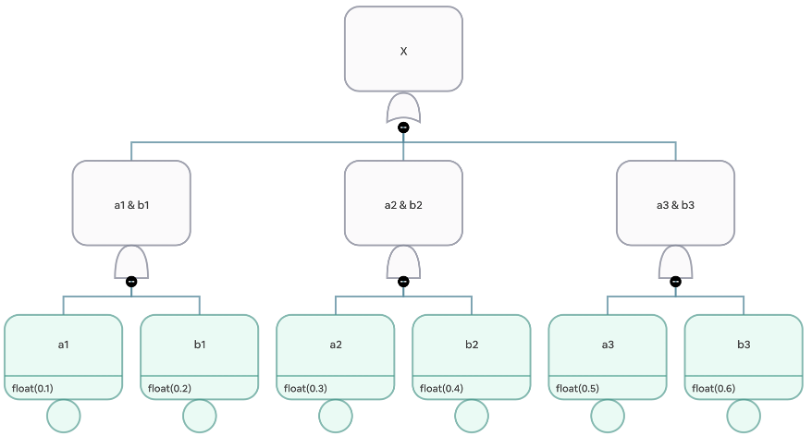
\includegraphics[width=0.5\textwidth]{1_concepts/ft.png}
    \caption{Fault tree with 6 basic events, top event $X = (a_1\bigwedge b_1) \bigvee (a_2\bigwedge b_2) \bigvee (a_3\bigwedge b_3)$}
    \label{fig:ft}
\end{figure}
\begin{itemize}
  \item A Fault Tree describes how a top event (system failure) can result from lower-level component or subsystem failures.
  \item Internal gates (AND, OR, \(k\)-of-\(n\), etc.) combine events in logical fashion:
    \[
      \text{Output} \;=\;
      \begin{cases}
         \bigwedge_{i=1}^k e_i, & \text{(AND)}\\
         \bigvee_{i=1}^k e_i, & \text{(OR)}\\
         \dots
      \end{cases}
    \]
  \item Basic events (BEs) in the leaves have assigned probabilities \(p(b)\).  Independence often assumed unless modeling common-cause failures.
  \item The top event failure probability can be written as:
    \begin{equation}
    \label{eq:top_event_probability_slides}
    \Pr[\text{Top Fail}] \;=\; \sum_{S \subseteq \,\mathcal{B}} 
      \Bigl[
        \pi_{F}(S, \text{Top}) 
        \prod_{b\in S} p(b)\prod_{b\notin S}[1 - p(b)]
      \Bigr].
    \end{equation}
\end{itemize}
\end{frame}

\begin{frame}[t, allowframebreaks]
\frametitle{Linking Event Trees and Fault Trees in PRA}
\begin{itemize}
  \item Real systems often combine:
    \begin{itemize}
      \item Forward branching dynamics via Event Trees (ET).
      \item Subsystem or component reliability logic via Fault Trees (FT).
    \end{itemize}
  \item An event tree branch may call a specific FT top event to collect system failure or success.
  \item Conversely, a fault tree output may feed back into an event tree branch as an initiating event or functional node outcome.
  \item This multi-level interconnection \(\implies\) a need for a unified model capturing both forward branching (ET) and hierarchical failure logic (FT).
\end{itemize}
\end{frame}

\begin{frame}[t, allowframebreaks]
\frametitle{Probabilistic Directed Acyclic Graph (PDAG)}
\begin{itemize}
  \item A PDAG is a Directed Acyclic Graph whose edges carry either:
    \begin{itemize}
      \item Conditional probabilities (e.g., for event tree branches).  
      \item Logical dependencies (e.g., for fault tree gates).
    \end{itemize}
  \item Nodes may include:
    \begin{itemize}
      \item Basic events (BEs) with known probabilities.
      \item ET or FT intermediate events storing partial results.
      \item Any top-level node (e.g., a final end-state) with no children.
    \end{itemize}
  \item The absence of cycles guarantees consistent flow from initial seeds (basic events, initiating events) to final outcomes.
  \item PDAG forms the structural backbone for bridging scenario-based expansions with gate-based logic in a single coherent representation.
\end{itemize}
\end{frame}

\subsection{Probabilistic Circuits Overview}
\begin{frame}[t, allowframebreaks]
\frametitle{Probabilistic Circuits: A Brief Overview}
    \begin{figure}[h]
    \centering
    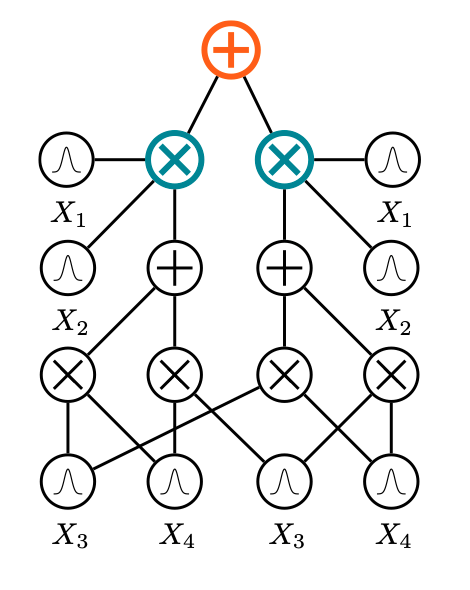
\includegraphics[height=0.5\textheight]{1_concepts/pc.png}
    \caption{Probabilistic circuit with 4 inputs $X_i$, product gates (blue), sum gate (orange)}
    \label{fig:pc}
\end{figure}
\end{frame}

\begin{frame}[t, allowframebreaks]
\begin{itemize}
  \item A \textbf{probabilistic circuit} is a directed acyclic graph (DAG) that encodes a joint probability distribution through \emph{sum-gates} and \emph{product-gates}.
  \item \textbf{Sum-gates} approximate mixture distributions:
    \[
      p_v(\mathbf{x})
      \;=\;
      \sum_{u\in \operatorname{ch}(v)} \theta_{v,u}\,p_u(\mathbf{x}),
      \quad
      \text{with }
      \sum_{u\in \operatorname{ch}(v)} \theta_{v,u} = 1.
    \]
    Each child distribution is weighted by a nonnegative parameter \(\theta_{v,u}\).
  \item \textbf{Product-gates} factorize independent variable sets:
    \[
      p_v(\mathbf{x})
      \;=\;
      \prod_{u\in \operatorname{ch}(v)} p_u\bigl(\mathbf{x}_{u}\bigr),
    \]
    assuming disjoint subsets of variables for each child \(u\).
  \item \textbf{Leaf nodes} (inputs) often correspond to known base distributions. When evaluated upward through the DAG, each internal node yields its own distribution, culminating in a root node that represents the full model.
  \item \textbf{Key motivation}:
    \begin{itemize}
      \item Tractable inference: evaluation and certain marginal or conditional queries can be performed in time proportional to circuit size.  
      \item Decomposability and modularity: separate, interpretable substructures that can be reused or combined for large-scale systems.
    \end{itemize}
\end{itemize}
\end{frame}

\subsection{PRA PDAGs to Probabilistic Circuits}
\begin{frame}[allowframebreaks]
\frametitle{Compiled PRA Graphs are PDAGs}
\begin{itemize}
  \item A unified PRA model can be viewed as
    \[
      \mathcal{M} 
      \;=\;
      \langle 
        \mathcal{V},\,\mathcal{A},\, \{p(b)\},\, \{\theta_{u\to v}\},\,\pi_{F}
      \rangle,
    \]
    where \(\mathcal{V}\) includes basic events, ET nodes, and FT gates, and \(\mathcal{A}\) is the acyclic edge set.
  \item Event-tree edges carry transitional probabilities \(\theta_{u\to v}\) summing to 1 from each node.
  \item Fault-tree nodes embed Boolean logic \(\pi_F\) that checks if inputs fail under a subset of basic events.
  \framebreak
  \item This PDAG perspective:
    \begin{itemize}
      \item Ensures systematic accounting of all scenario paths and subsystem logic.
      \item Aligns naturally with tractable Probabilistic Circuits, since each node’s distribution/function can be embedded in a sum-product style DAG.
      \item Offers a foundation for efficient Monte Carlo or advanced inference methods.
    \end{itemize}
    \vspace{6pt}
    \item Ongoing work to bridge PRA PDAG semantics with Probabilistic Circuits:
    \begin{itemize}
      \item PDAGs can be transformed to equivalent canonical forms (there are tradeoffs).
    \end{itemize}
\end{itemize}
\end{frame}